\chapter{Voltage unbalance on domestic networks}\label{BASIC:sec:main}

In this chapter the basic topics of the thesis are discussed, as components for further understanding. First the phenomena of voltage unbalance on small distribution networks are shown and the ambiguities though the development of the concept, and at the end the norm currently being in use in the industry. It would be shown how many definitions are currently in use, thus the introduced ambiguity of definition, further validating the proposal in section \ref{VUB:sec:Geom}.\\
Next a necessary glimpse of power electric background is given to invite to the viewpoint of the modeling and problem breakdown of power converter. The section would introduce the background of current source switching devices with forced commutation, since control based on external situations or according to a cost function is eminent. After the single phase method shall be described, DC-DC conversion would be shown, since in section \ref{VUB:sec:Compensation} non-zero mean asymmetrical power injection was required. The section closes with the three phase rectifier example, for contributing the understating of the modeling in section \ref{EMPC:sec:Modeling}.\\
Lastly the basis of controller structures, shall be shown, applied in the thesis. These are the APPS (asynchronous parallel pattern search) method (used in section \ref{VUB:sec:Optimization}) and constrained model based predictive control (MPC) is to be described with the end with the explicit partition of the state space (explicit MPC applied in section \ref{EMPC:sec:DCside}) for a computationally efficient approach.

	\section{Definitions of voltage unbalance}\label{BASICUNB:sec:DefinitionsofUNB}

%\textbf{(Mostly) from Wikipedia:}\\
In a symmetric three-phase power supply system, three conductors each carry an alternating current of the same frequency and voltage amplitude relative to a common reference but with a phase difference of one third of a cycle between each. The common reference is usually connected to ground and often to a current-carrying conductor called the neutral. Due to the phase difference, the voltage on any conductor reaches its peak at one third of a cycle after one of the other conductors and one third of a cycle before the remaining conductor. This phase delay gives constant power transfer to a balanced linear load.\\
In general symmetric three-phase systems described, are simply referred to as three-phase systems because, although it is possible to design and implement asymmetric three-phase power systems (i.e., with unequal voltages or phase shifts), they are not used in practice because they lack the most important advantages of symmetric systems. In a three-phase system feeding a balanced and linear load, the sum of the instantaneous currents of the three conductors is zero. In other words, the current in each conductor is equal in magnitude to the sum of the currents in the other two, but with the opposite sign. The return path for the current in any phase conductor is the other two phase conductors.\\
Constant power transfer and cancelling phase currents would in theory be possible with any number (greater than one) of phases, maintaining the capacity-to-conductor material ratio that is twice that of single-phase power. However, two-phase power results in a less smooth (pulsating) torque in a generator or motor (making smooth power transfer a challenge), and more than three phases complicates infrastructure unnecessarily.\\
Three-phase systems may also have a fourth wire, particularly in low-voltage distribution. This is the neutral wire. The neutral allows three separate single-phase supplies to be provided at a constant voltage and is commonly used for supplying groups of domestic properties which are each single-phase loads. The connections are arranged so that, as far as possible in each group, equal power is drawn from each phase. Further up the distribution system, the currents are usually well balanced. Transformers may be wired in a way that they have a four-wire secondary but a three-wire primary while allowing unbalanced loads and the associated secondary-side neutral currents \cite{von2006electric}.

\subsection{Phenomena of voltage unbalance}\label{BASICUNB:sec:PhenomenafUNB}

In a domestic network, three-phase electric power systems have at least three conductors carrying alternating voltages that are offset in time by one-third of the period. A three-phase system may be arranged in delta  or star. A star system allows the use of two different voltages from all three phases, such as a 230/400 V system which provides 230 V between the neutral (center hub) and any one of the phases, and 400 V across any two phases displayed on Fig.\ref{BASICUNB:fig:UnbWave}. The definition is the following:
	
			\begin{equation}
        \begin{array}{rcl}
            \vec{V}_a&=&\hat{V}\,sin(\theta)\\
						\vec{V}_b&=&\hat{V}\,sin(\theta+\frac{4}{3}\pi)\\
						\vec{V}_c&=&\hat{V}\,sin(\theta+\frac{2}{3}\pi),\\
        \end{array}
        \label{BASICUNB:equ:Definition}
    \end{equation}
	
	where $\vec{V}_a,\,\vec{V}_b,\,\vec{V}_c$ are the phase voltage vectors, $\hat{V}$ is the voltage peak, and $\theta$ is the phase angle. Voltage unbalance a phenomena where the three phase voltages differ in amplitude normal 120 degree phase relationship shown in Fig.\ref{BASICUNB:fig:UnbPhasor}. In most cases both are happening at the same time. This includes unequal voltage magnitudes at the fundamental frequency, either under, or over voltage, at the fundamental phase angle deviation.
	
	\begin{figure}[h!]
     \centering
		\begin{subfigure}[b]{0.49\textwidth}
         \centering
         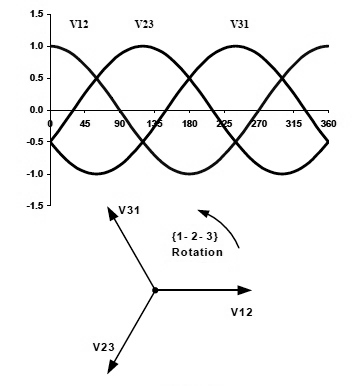
\includegraphics[width=\textwidth]{Unblance_EPS_Pics/Three-phase-voltage-system_gray.png}
         \caption{Three phase sine wave of network voltage.}
         \label{BASICUNB:fig:UnbWave}
     \end{subfigure}
		\hfill
     \begin{subfigure}[b]{0.49\textwidth}
         \centering
         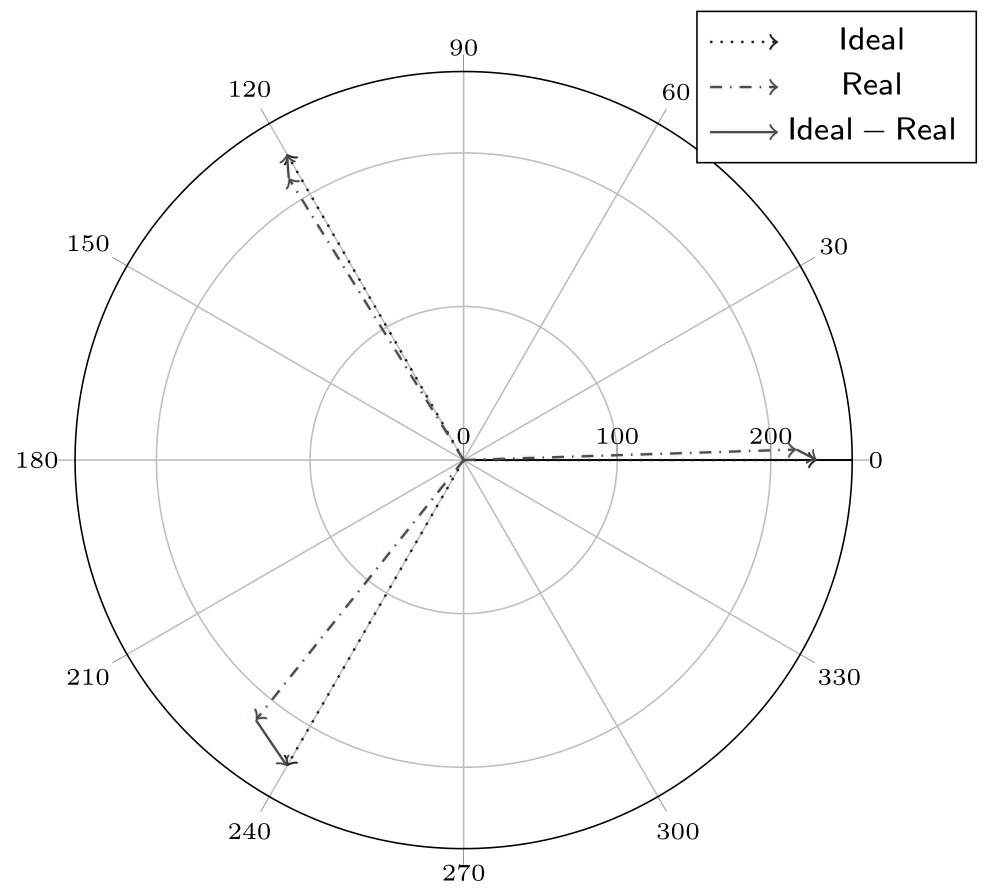
\includegraphics[width=\textwidth]{Unblance_EPS_Pics/PhasorGrayscale.jpg}
         \caption{The three phase voltage phasor whith $Ideal$ and $Real$ voltage vectors.}
         \label{BASICUNB:fig:UnbPhasor}
     \end{subfigure}
        %\caption{BASICUNB:fig:UnbPhasor}
        \label{BASICUNB:fig:UnbPhasor_all}
\end{figure}
	
	This is observed as a frequently cited power quality issue in low-voltage domestic distribution networks and in systems that supply large single phase loads distributed unevenly among the phases. Effects of voltage unbalance are complex, but can be categorized as structural or functional. The former refers to the asymmetry in the three-phase impedances of transmission lines, cables, transformers, etc. It occurs because it is neither economical nor necessary to maintain distribution system with perfectly symmetrical impedances. The latter refers to uneven distribution of power consumption over the three phases. Although the term voltage unbalance is unambiguous, the root phenomenon may be various as well as the standard norms used to measure unbalance. All of these different indicators measure voltage unbalance but each of them does it in a different way. In this section a detailed explanation is presented about the types of currently used method for indication.
	
	\subsection{Types of voltage deviations and norms}\label{BASICUNB:sec:DefinitionsofUNB}

        Voltage unbalance is not a straightforward term. To understand the concept, unbalance is when on a given frequency (mostly fundamental frequency) voltage vectors (phase or line depending on the definition) deviating from the ideal in terms of length or angle. The first fall in to the category of unbalance, namely any kind of phase deviations, and unbalanced amplitude deviations, and balanced amplitude deviations, like under-voltage. There are many different technological causes with more or less practical importance. The following conditions are examined and tested in the sequel:
        \begin{description}
        \item[Single phase under-voltage unbalance]  If there is a single phase uncompensated overload in the system, the voltage in the overloaded phase will be lower than the other two.
        \item[Two phase under-voltage unbalance]  Two of the three phases are overloaded without compensation, the two overloaded phases will have higher voltage drop than the third phase.
        Balanced three phase under-voltage]  The loads of all three phases are overloaded in an unbalanced manner.
        \item[Unbalanced single phase angle]  If the three phase voltage amplitudes are balanced but the relative angles between them (ideally it should be equal to $\pm120$ degree). It is assumed, that $V_a$ would be the reference. If one of the other two phase angles is deflected, unequal displacement.
        \item[Unbalanced two phase angles displacement] Similar to the single phase angle unbalance, if the other two phase angles are both deflected, then unequal angle displacement in two phase angles occurs.
        \end{description}
        An indicator of the voltage unbalance is supposed to measure the extent of unbalance but it is not expected to classify between the above types.
	
	\subsection{Non standardized approximation formulas}\label{BASICUNB:sec:ApproxFormula}
	
	Up to now, the following definitions have not been adopted by any standard or rule to indicate the degree of voltage unbalance, but used by various manufacturers. Firstly based on \cite{eugene1986new} recommended by the CIGRE (International Council on Large Electric Systems, in French: Conseil International des Grands Réseaux Électriques), the voltage unbalance is determined with:
	
	\begin{equation}
        \begin{array}{rcl}
            VUFactor&=&\frac{\sqrt{{1-\sqrt{3-6\frac{V_{ab}^4+V_{bc}^4+V_{ca}^4}{\left(V_{ab}^2+V_{bc}^2+V_{ca}^2\right)^2}}}}}{1+\sqrt{3-6\frac{V_{ab}^4+V_{bc}^4+V_{ca}^4}{\left(V_{ab}^2+V_{bc}^2+V_{ca}^2\right)^2}}}\\
						%\textnormal{where},&&\\
						%\upsilon&=&\frac{V_{ab}^4+V_{bc}^4+V_{ca}^4}{\left(V_{ab}^2+V_{bc}^2+V_{ca}^2\right)^2},					
        \end{array}
        \label{BASICUNB:equ:CIRGE}
    \end{equation}
		
		where, $\{V_{ab},V_{bc},V_{ca}\}$ are the line-to-line voltages. Note, that the CIRGE variant has no distinct notation, as such it would be indicated as $VUFactor$ in this thesis. Moreover, the author of \cite{robert1992assessing} recommends two more variants, based on manufacturer recommended"standards":
		
		\begin{equation}
        \begin{array}{rcl}
            VU&=&\frac{82\cdot\sqrt{(V_{ab}-V_{avg_{line}})^2+(V_{bc}-V_{avg_{line}})^2+(V_{ca}-V_{avg_{line}})^2}}{V_{avg_{line}}}\times100\\					
        \end{array}
        \label{BASICUNB:equ:VU}
    \end{equation}
		
		\begin{equation}
        \begin{array}{rcl}
            VUR&=&\frac{max\left( |V_{ab}-V_{bc}|,|V_{bc}-V_{ca}|,|V_{ca}-V_{ab}| \right)}{V_{avg_{line}}}\times100,\\				
        \end{array}
        \label{BASICUNB:equ:VUR}
    \end{equation}
		
		where the mean of line voltages is noted by $V_{avg_{line}}=\frac{V_{ab}+V_{bc}+V_{ca}}{3}$.
		This formulas were created with the intention to avoid the use of the complex algebra in symmetrical components and give
a good approximation of the later described $VUF$ standard. With the indicator of \ref{BASICUNB:equ:VU}, and as well as \ref{BASICUNB:equ:VUR}. It is worth noticing, that only the voltage magnitude unbalance is reflected, completely ignoring Fortescue's method of symmetrical components \cite{fortescue1918method} (shall presented later in the thesis), which considers negative sequence components as harmful on electric equipment and yield. Later it will be shown that other methods try to push the same methodology, until the currently used norm ($VUF$) is used.

	
	\subsection{LVUR}\label{BASICUNB:sec:LVUR}
	
	One of the first voltage unbalance in percent is defined by the National Electrical Manufacturers Association (NEMA) \cite{bonnett1997understanding} is defined  as the ratio of the maximum voltage deviation from the average line voltage magnitude to the average line-voltage magnitude.
	
\begin{equation}
        \begin{array}{rcl}
            LVUR&=&\frac{\max\left( |V_{ab}-V_{avg_{line}}|,|V_{bc}-V_{avg_{line}}|,|V_{ca}-V_{avg_{line}}| \right)}{V_{avg_{line}}}\times100\\			
        \end{array}
        \label{BASICUNB:equ:LVUR}
    \end{equation}
		
		The LVUR assumes that the average voltage is always equal to the rated value, which is 480 volts for the US three-phase systems, and it works only with magnitudes. Phase angles are not considered in this definition.
	
	\subsection{PVUR}\label{BASICUNB:sec:PVUR}
	
	The next phase voltage unbalance in percent described in IEEE standard $141.$ \cite{IEEE_141_35071} (derived from \cite{IEEE_112_8635630}), is $PVUR_{IEEE-141}$. It is defined as the ratio of the maximum voltage deviation of phase voltages from the average phase-voltage magnitude to the average phase voltage magnitude. In various fields, LVUR and $PVUR_{IEEE-141}$ are commonly used to estimate the degree of voltage unbalance due to simplicity of calculation. The two unbalance factors mentioned above cannot completely reflect system voltage unbalance effects, such as the phase displacements of unbalanced voltages.
	
	\begin{equation}
        \begin{array}{rcl}
            PVUR_{IEEE-141}&=&\frac{\max\left( |V_{a}-V_{avg_{phase}}|,|V_{b}-V_{avg_{phase}}|,|V_{c}-V_{avg_{phase}}| \right)}{V_{avg_{phase}}}\times100,\\
        \end{array}
        \label{BASICUNB:equ:PVUR-141}
    \end{equation}

where the voltages $\{V_{a},V_{b},V_{c}\}$ denotes the phase-to-neutral voltages, and $V_{avg_{phase}}=\frac{V_{a}+V_{b}+V_{c}}{3}$.
The second variant is, $PVUR_{IEEE-936}$, mentioned in \cite{IEEE_936_29053} is defined as the ratio of the difference between the highest and the lowest phase-voltage magnitude to the average phase-voltage magnitude. Therefore, the numerical values of voltage balance quantified by $PVUR_{IEEE-936}$ are generally larger than those of $PVUR_{IEEE-141}$ and LVUR.

\begin{equation}
        \begin{array}{rcl}
            PVUR_{IEEE-936}&=&\frac{\max\left( |V_a|,|V_b|,|V_c| \right)-min\left( |V_a|,|V_b|,|V_c| \right)}{V_{avg_{phase}}}\times100,\\					
        \end{array}
        \label{BASICUNB:equ:PVUR-936}
    \end{equation}
		
The number of possible combinations of three phase or line voltages that satisfy the definitions of voltage unbalance mentioned above will become infinite as only the magnitudes of voltages are considered.	
		
	
	\subsection{VUF and CVUF}\label{BASICUNB:sec:VUFCVUF}
	
	The voltage unbalance factor ($VUF$) was defined by the International Electrotechnical Commission \cite{pillay2001definitions}, \cite{dugan1996electrical}. From the theorem of symmetrical components \cite{fortescue1918method}, voltage unbalance can be considered as a phenomenon that positive sequence voltage  ($V_p$) is disturbed by negative  ($V_n$) and zero-sequence ($V_0$) voltages:
	
	\begin{equation}
        \begin{array}{rcl}
            \begin{bmatrix}
						V_0\\
						V_p\\
						V_n\\
						\end{bmatrix}&=&
						\frac{1}{3}\begin{bmatrix}
						1&1&1\\
						1&\upsilon&\upsilon^2\\
						1&\upsilon^2&\upsilon\\
						\end{bmatrix}\cdot
						\begin{bmatrix}
						V_a\\
						V_b\\
						V_c\\
						\end{bmatrix},\\
        \end{array}
        \label{BASICUNB:equ:symmetry}
    \end{equation}
	
	Where $\upsilon=e^{2j\pi/3}$ is the Fortesque operator. From that the formula of $VUF$ can be expressed as:
	
	
	\begin{equation}
        \begin{array}{rcl}
            VUF&=&\left|\frac{V_n}{V_p}\right|\times100,\\					
        \end{array}
        \label{BASICUNB:equ:VUF}
    \end{equation}

    \begin{figure}[h]
         \centering
         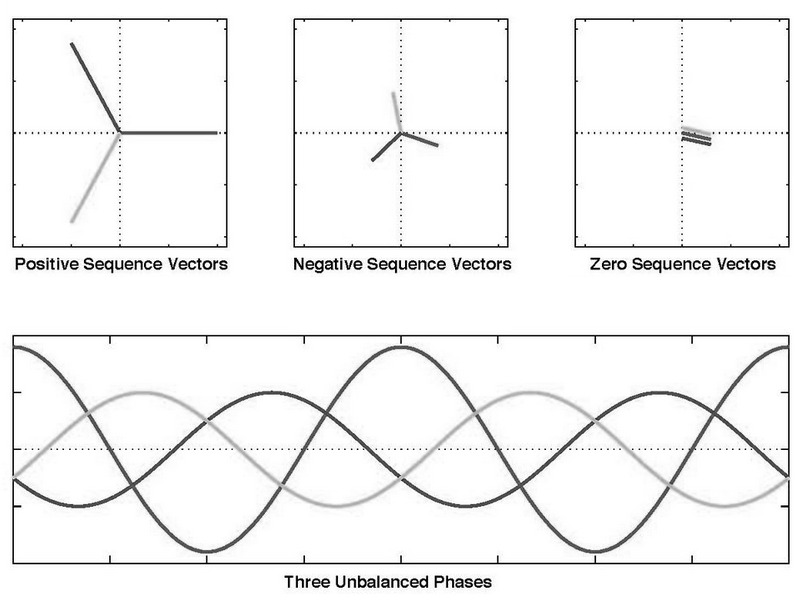
\includegraphics[width=.7\textwidth]{Unblance_EPS_Pics/Symmetrical_components_gray.jpg}
         \caption{Simplified graphical display of symmetrical components.}
         \label{BASICUNB:fig:symmetrical_simple}
     \end{figure}
	
This norm is currently in use world wide for voltage unbalance indication. The main focus in on the negative sequence component $V_n$, on which many studies attributes importance of the cause of negative effects the voltage unbalance causes.\\
	As such, three-phase electric loads without path through the neutral, negative-sequence voltage is the primary cause of voltage unbalance. Normally, positive-sequence component of three-phase voltages is very close to rated value. If expressed in per-unit quantities, the positive-sequence voltage will be very close to $1.0$ p.u., and the corresponding negative-sequence voltage will be very close to the $VUF$. Thus, the $VUF$ can indeed be considered as the negative-sequence component in per-unit.	This explains the advantage of using the VUF as an index for analyzing the effects of voltage unbalance considering the phase deviations.
	An extension of the VUF is the complex voltage unbalance factor ($CVUF$) that is defined by the ratio of the negative-
sequence voltage phasor to the positive-sequence voltage phasor studied in \cite{wang2000analytical}, and \cite{pierrat1987unbalance}. The CVUF is a complex quantity having the magnitude and the angle. Although the CVUF has not yet been widely used by practicing engineers, it has been proposed in some studies (e.g., \cite{wang2001analysis}, \cite{singh2007some}, \cite{chen2013examination}) due to its richness of information on unbalance. The formula of $CVUF$ is similar to $VUF$:

\begin{equation}
        \begin{array}{rcl}
            k_v&=&\frac{V_n}{V_p}=k_v\cdot e^{j\theta_v}=k_v\angle\theta_v,\\					
        \end{array}
        \label{BASICUNB:equ:CVUF}
    \end{equation}
		
		where $k_v$ is the magnitude and $\theta_v$ is the angle of $CVUF$.
		
			It can be observed, that the previously mentioned norms \ref{BASICUNB:equ:CIRGE}, \ref{BASICUNB:equ:VU}, \ref{BASICUNB:equ:VUR}, \ref{BASICUNB:equ:LVUR}, \ref{BASICUNB:equ:PVUR-141}, \ref{BASICUNB:equ:PVUR-936}, and \ref{BASICUNB:equ:VUF}  indicate different values for a single case with various correlations. The first two standard indicators, $PVUR_{IEEE-936}$ and $PVUR_{IEEE-141}$, ignore the $\pm120$ degree phase difference unbalance and only take the amplitudes into account. Additionaly, the zero-sequence components never present in the line-to-tine voltages regardless of the level of unbalance, only phase-to-neutral voltages. It has been proven, that these components are unelectable in some cases like bridge control of converters \cite{betz2006symmetry}, or synchronous machine diagnosis \cite{hang2015online}.\\
			The actual state of the art definition in use, $VUF$, is sensitive to the phase difference unbalance. Lastly $CVUF$ considers also phase and magnitude of the voltage unbalance, but the two units are hard to merge together as the optimization cost of a cost function. Moreover, these definitions ignore zero sequence components and harmonic distortion that are always present in three-phase four-wire systems \cite{bina2011three}.
		
% =========== SECTION MIGRATED TO INTRODUCTION -->

			%\section{Effects of voltage unbalance}
			%
			%Many power systems, voltage parameters change over time. Variation of power quality disturbances leads to thermal transients in electrical machines. This problem can be especially important in the case of low-power machines, because they have shorter time constants than high-power ones. The rate of thermal responses of a machine also significantly depends on the type of power quality disturbances. Voltage unbalance can cause  machine  overheating  within  a  mere  few  minutes. Furthermore,  fluctuating  unbalance  could  cause  an  extraordinary rise  in  windings  temperature  and  additional  thermo-mechanical stress.  Consequently,  voltage  unbalance  is  found  to  be  more harmful to induction motors than the results from previous works \cite{gnacinski2019induction}. Additionally beside the heat factor, voltage unbalance can cause increased reactive power \cite{savaghebi2012secondary}, various copper loss \cite{siddique2004effects} torque pulsation in electric motors \cite{brekken2005control} have been studied.

%	NO SUMMARY REQUIRED
	

